\documentclass[12pt]{report}
\usepackage[a4paper, total={6.5in, 9.5in}]{geometry}
\usepackage{graphicx}
\usepackage{biblatex}
\usepackage{fancyhdr}
\usepackage[style=iso]{datetime2}
\usepackage{parskip}
\usepackage{titlesec}
\usepackage{csquotes}
\usepackage{amsmath}
\usepackage[swedish]{babel}

\titleformat{\chapter}[display]
    {\normalfont\LARGE\bfseries}
    {}
    {0pt}
    {}
\titlespacing{\chapter}
    {0pt}
    {0pt}
    {0pt}

\titleformat{\section}[display]
    {\normalfont\Large\bfseries}
    {}
    {0pt}
    {}
\titlespacing{\section}
    {0pt}
    {0pt}
    {0pt}

\titleformat{\subsection}[display]
    {\normalfont\large\bfseries}
    {}
    {0pt}
    {}
\titlespacing{\subsection}
    {0pt}
    {0pt}
    {0pt}

\titleformat{\subsubsection}[display]
    {\normalfont\normalsize\bfseries}
    {}
    {0pt}
    {}
\titlespacing{\subsubsection}
    {0pt}
    {0pt}
    {0pt}

\titleformat{\paragraph}[display]
    {\normalfont\small\bfseries}
    {}
    {0pt}
    {}
\titlespacing{\paragraph}
    {0pt}
    {4pt}
    {2pt}


\addbibresource{references.bib}

\def\title{Rapportmall IV steg 2}
\def\course{XXX000 Kursnamn (se kursplan)}

\begin{document}

\begin{titlepage}
    \thispagestyle{plain}
    \fancypagestyle{plain}{
        \renewcommand{\headrulewidth}{0pt}

        \fancyfoot[C]{}

        \fancyfoot[L]{
            REDOVISNING

            \course

            Institutionen för ingenjörsvetenskap
        }
    }

    \begin{minipage}{0.3\textwidth}
        \vspace{-1cm}
        
\includegraphics[width=\textwidth]{images/logo}
    \end{minipage}
    \hfill
    \begin{minipage}{0.4\textwidth}
        \vspace{-3cm}
        \begin{flushright}
        Inlämningsdatum: \today
        \end{flushright}
    \end{minipage}

    \vspace{5cm}

    \Huge
    \textbf{\title}

    \Large
    \vspace{1cm}
    Eventuellt gruppnummer

    Författare 1

    Författare 2

    Författare 3

    Författare 4
\end{titlepage}


\setcounter{secnumdepth}{0}
\pagenumbering{roman}

\newpage

\thispagestyle{plain}

\section{Förord}
I föreliggande rapportall visas grundstrukturen hos en förenklad akademisk
rapport samt vägledning till den typografiska utformningen, medan anvisningar
kring språkhantering, disposition och utformning tas upp i dokumentet
\textit{Anvisningar skrivprogression steg 2}.

Mallen är framtagen med hjälp av \LaTeX och testad mot 
\verb|texlive|-kompilatorn \verb|pdflatex| med \verb|bibtex|-stöd via
\verb|biber|.

Ta bort förekommande blå överstrykningar när markerad text har ändrats. 

\vspace{1cm}

Trollhättan, februari 2024

Hampus Avekvist

\newpage

\section{Sammanfattning}
Sammanfattning får inte vara längre än att den tillsammans med
dokumentinformationen nedan får plats på en och samma sida. 

\vfill
\begin{table}[ht!]
    \centering
    \begin{tabular}{|l l|}
        \hline
        Datum: &\today \\
        Författare: &Författare 1, Författare 2, Författare 3, Författare 4 \\
        Kurs: &\course \\
        Kursansvarig: &Arthur Dent och Ford Prefect \\
        & Högskolan Väst, Institutionen för ingenjörsvetenskap \\
        \hline
    \end{tabular}
\end{table}

\pagestyle{fancy}
\fancyhf{}
\fancyhead[C]{\title}
\fancyfoot[C]{\thepage}

\setcounter{secnumdepth}{3}
\tableofcontents
\thispagestyle{fancy}

\titleformat{\chapter}[display]
    {\normalfont\LARGE\bfseries}
    {}
    {0pt}
    {\thechapter\ }

\titleformat{\section}[display]
    {\normalfont\Large\bfseries}
    {}
    {0pt}
    {\thesection\ }

\titleformat{\subsection}[display]
    {\normalfont\large\bfseries}
    {}
    {0pt}
    {\thesubsection\ }

\titleformat{\subsubsection}[display]
    {\normalfont\normalsize\bfseries}
    {}
    {0pt}
    {\thesubsubsection\ }


\newpage
\pagenumbering{arabic}

\chapter{Rubrik nivå 1}
Sidorna i huvuddelen numreras löpande med början på 1. De sidor som föregår
huvuddelen (sammanfattning och innehållsförteckning) numreras separat med
romerska siffror. 

\section{Rubrik nivå 2}
I föreliggande rapportmall används huvudsakligen teckensnittet
\textit{Garamond} för löpande text och \textit{Arial} för rubriker. För
symboler som konstanter och variabler skall teckensnittet \textit{Cambria}
användas, såväl i ekvationer som när de skrivs i den löpande texten. För
grekiska tecken används teckensnittet \textit{Symbol}. För listning av
programkod eller liknande rekommenderas att ett teckensnitt med fast
teckenbredd används, exempelvis \textit{Courier}.

\subsection{Rubrik nivå 3}
I mallen finns formatmallar för stycken av olika typ, exempelvis används
formatmallen \textit{Brödtext} (eng: \textit{Body Text}) för alla stycken
som är löpande text och \textit{Rubrik 1}, \textit{Rubrik 2}, ... (eng:
\textit{Heading 1}, \textit{Heading 2}, ...) för rubriker på olika nivåer.

Följande stycke är ett så kallat blockcitat formaterat som \textit{Citat}
(eng: \textit{Quote}):

\begin{displayquote}
    There is an art to flying, or rather a knack. Its knack lies in learning
    to throw yourself at the ground and miss. ... Clearly, it is this
    second part, the missing, that presents the difficulties. (Adams, 1982)
\end{displayquote}

Nedan följer exempel där formatmallen \textit{Beskrivning} (eng:
\textit{Caption}) används på förklaringarna till \ref{tab:fruits} och 
\ref{fig:flowchart}. I \LaTeX finns även möjlighet att infoga automatisk
numrering och hänvisning genom att använda \verb|\ref| och \verb|\label|.

\begin{table}[ht!]
    \label{tab:fruits}
    \centering
    \caption{Två olika frukters egenskaper.}
    \begin{tabular}{|l|l|l|l|}
        \hline
        & \textbf{Form} & \textbf{Färg} & \textbf{Smak} \\
        \hline
        \textbf{Banan} & Långsmal & Gul & Söt \\
        \hline
        \textbf{Citron} & Rund & Gul & Sur \\
        \hline
    \end{tabular}
\end{table}

\begin{figure}[ht!]
    \label{fig:flowchart}
    \centering
    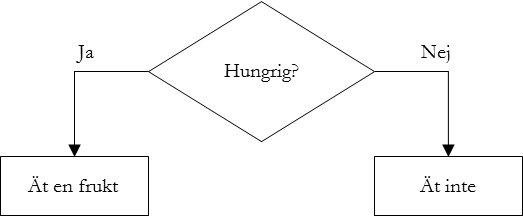
\includegraphics[width=7cm]{images/flowchart}
    \caption{Ett enkelt flödesschema}
\end{figure}

\subsubsection{Rubrik nivå 4}
I mallen är avsnitt på nivå 4 numrerade, men numreringen med fyra nummer
kan i många fall upplevas som förvillande och bör normalt undvikas. Det
rekommenderas att istället använda formatmallen \textit{Rubrik 5} (eng:
\textit{Heading 5}) på dessa rubriker, se följande avsnittsrubrik. 

\paragraph{Rubrik nivå 5}
För att ekvationer ska få rätt utseende och samtidigt kunna numreras används
miljön \verb|equation|. \LaTeX formatterar automatiskt så ekvationen
centreras och numreras. 

\begin{equation}
    \label{eq:integral}
    I_0 = \frac{1}{T}\int_0^T i(t)dt
\end{equation}

I kontrast till Microsoft Word behövs här inga tabeller för formatteringen
och numreringen utan \LaTeX har inbyggt stöd. Vill man ha en ekvation
utan numrering kan man använda miljön \verb|align*|. 

\begin{align*}
    e^{i\pi}-1=0
\end{align*}

\LaTeX hanterar numreringen automatiskt och för att referera till en
ekvation kan man lägga in \verb|label| och använda \verb|\ref| som detta:
\ref{eq:integral}. 

\chapter{Rubrik nivå 1}
Rubriker på nivå 1 (kapitelrubriker) ska alltid stå överst på sidan, det
vill säga de ska föregås av sidbrytning. Rubriker på nivå 2, 3, etc
(avsnittsrubriker) skall normalt inte föregås av sidbrytning. 

\section{Rubrik nivå 2}
Brödtext

\section{Rubrik nivå 2}
Brödtext

\subsection{Rubrik nivå 3}
Brödtext

\subsection{Rubrik nivå 3}
Brödtext

\section{Rubrik nivå 2}
Brödtext

\subsection{Rubrik nivå 3}
Brödtext

\subsection{Rubrik nivå 3}
Brödtext

\newpage

\titleformat{\chapter}[display]
{\normalfont\LARGE\bfseries}
{}
{0pt}
{}
\titlespacing*{\chapter}
{0pt}
{0pt}
{0pt}

\nocite{*}
\printbibliography[
    heading=bibintoc,
    title={Referenser}
    ]
    \thispagestyle{fancy}

    \appendix

    \titleformat{\chapter}[display]
    {\normalfont\LARGE\bfseries}
    {}
    {0pt}
    {Bilaga \thechapter:\ }
    \titlespacing*{\chapter}
    {0pt}
    {0pt}
    {0pt}

    \chapter{Rubriktext}
    Bilagornas rubriker ska ha formatmallen \textit{Rubrik 7} (eng:
    \textit{Heading 7}) för att de ska synas på rätt sätt i innehållsförteckningen.
    Bilagerubriker inleds alltid med \textbf{Bilaga} \#: där \#=\textbf{A,B,C,...}.
    De ska alltid stå överst på sidan, det vill säga de ska föregås av sidbrytning.

    \chapter{Rubriktext}

\end{document}
